\documentclass{beamer}
\usepackage[utf8]{inputenc}
\usepackage{graphicx}
\author[Sowmya Vajjala]{Instructor: Sowmya Vajjala}

\title[LING 520]{LING 520: Computational Analysis of English}
\subtitle{Semester: FALL '16}

\date{25 August 2016}

\institute{Iowa State University, USA}
%%%%%%%%%%%%%%%%%%%%%%%%%%%

\begin{document}

\begin{frame}\titlepage
\end{frame}

\begin{frame}
\frametitle{Class outline}
\begin{itemize}
\item Why is NLP hard? %20 min
\item What are some common NLP tasks? %20 min
\item Assignment 1 overview %10min
\item Programming project demos %10 min
\end{itemize}
\end{frame}

\begin{frame}
\begin{center}
\Large Why is NLP hard?
\\ (what sort of issues pose problems for a computer?)
\end{center}
\end{frame}

\begin{frame}
\frametitle{Language is ambiguous}
\framesubtitle{Some ambiguous sentences}
\begin{itemize}
\item Newspaper headlines
\begin{itemize}
\item "Children make delicious snacks"
\item "Dead expected to rise"
\item "Republicans grill IRS chief over lost emails"
\end{itemize}
\item Normal, grammatical sentences can be ambiguous too:
\begin{itemize}
\item "I saw a man on a hill with a telescope."
\item "Look at the man with one eye"
\end{itemize}
\end{itemize}
We are not even talking about ambiguities involving speech or alternative interpretations due to stress/emphasis on some word.
\end{frame}

\begin{frame}
\frametitle{Some types of ambiguity}
\begin{enumerate}
\item Lexical ambiguity: due to multiple meanings or senses of word usage
\\ e.g., He stood near the \textbf{bank}
\item Structural ambiguity: due to syntactic structure
\\ e.g., I saw the man on the hill with telescope.
\item Semantic ambiguity: more interpretations possible
\\ e.g., John and Mary are married (to each other? or to different people?)
\item Referential ambiguity
\\ e.g., She dropped the \textit{plate} on the \textit{table} and broke \textbf{it}
\item Ambiguity due to the use of non-literal language
\\ e.g., Time flies like an arrow
\end{enumerate}
Good source to read more: \url{http://cs.nyu.edu/faculty/davise/ai/ambiguity.html}
\end{frame}

\begin{frame}
\frametitle{Ambiguity for humans}
\framesubtitle{this happened to me last night ...}
\begin{itemize}
\item "ISU sends out alert as devastating weed spreads in Iowa" - read a local newspaper headline. What did you understand?
\pause
\item My immediate reaction: Some new drug is circulating and ISU wants its students to be aware and not consume it. 
\pause
\item However, the actual news is about some poisonous wild plant, and the alert was issued by ISU weed and crop specialists to farmers.
\end{itemize}
... so some humans also cannot disambiguate certain things.
\end{frame}

\begin{frame}
\frametitle{"common" knowledge for humans}
Look at these two sentences:
\\ Dog bit man.
\\ Man bit dog.
\\ - For a computer, both of them are linguistically the same. We know only the first one is "normal" English sentence (I hope!) because we have "world knowledge".
\end{frame}

\begin{frame}
\frametitle{Language is creative}
Literary texts have their own language style: long sentences, neologisms, creative usage of words etc.
\end{frame}

\begin{frame}
\frametitle{Language can be complex to understand}
Legal documents, Writing style of some authors, propaganda materials, etc.
\end{frame}

\begin{frame}
\frametitle{Language is Diverse}
\framesubtitle{Some Examples}
\begin{itemize}
\item There are different types of text online: news, tweets, SMS, email, forum posts, speech transcripts etc.
\item Each genre has some specific characteristics of its own
\item NLP methods should generalize to all genres, and at the same time capture such specific characteristics
\item Example: a machine translation model created by training examples from European parliament speeches should also be able to translate casual day to day conversations.
\end{itemize}
\end{frame}

\begin{frame}
\frametitle{Other Issues}
\begin{itemize}
\item different text formats (pdf, doc, txt etc)
\item spelling variations
\item sarcasm
\item slang
\item using synonyms, paraphrases etc 
\end{itemize}
.. and so on.
\end{frame}

\begin{frame}
\frametitle{Languages are many}
.. and each language has its own special characteristics apart from similarities with other languages. NLP should handle both these aspects. 
\end{frame}

\begin{frame}
\frametitle{So, the summary is:}
perfect NLP is hard to achieve because of all these issues that come up when we start using computers to analyze language!
\end{frame}

%Ask some questions here?
\begin{frame}
\frametitle{Question Time}
\begin{itemize}
\item Apart from all these, what are some CALL specific problems for NLP? 
%grammatically incorrect sentences? 
\pause 
\begin{itemize}
 \item One issue I can think of: all NLP tools usually work under the assumption that there is only one standard way of writing in a given language, and everyone writes grammatically correct sentences.
\end{itemize}
\end{itemize}
\end{frame}

\begin{frame}
\begin{center}
\Large Some NLP tasks
\end{center}
\end{frame}

\begin{frame}
\frametitle{Let us take a small text snippet}
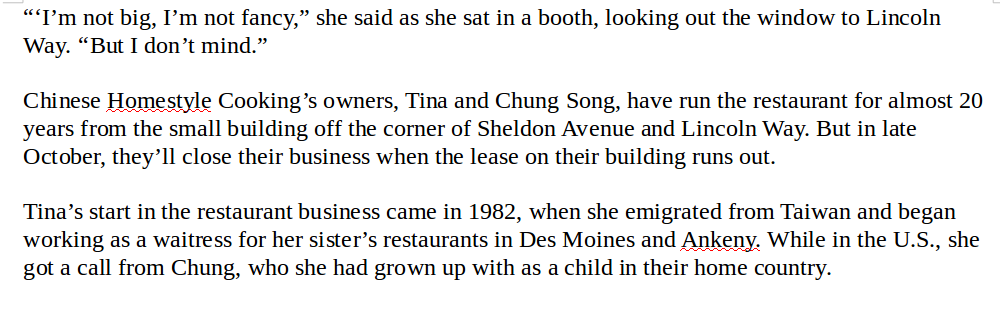
\includegraphics[width=0.9\textwidth]{Example.png}
\\ \footnotesize{Source: Ames Tribune (\url{http://goo.gl/zvx9Uw})}

\begin{enumerate}
\item When she says "I" in the first sentence, does she mean herself literally? \pause
\item What is she referring to? When will we know what is she referring to? \pause
\item Who is "She"? \pause
\item What is "home country" in the last sentence?  
\end{enumerate}
\end{frame}

\begin{frame}
\frametitle{More Questions}
\frametitle{Let us take a small text snippet}
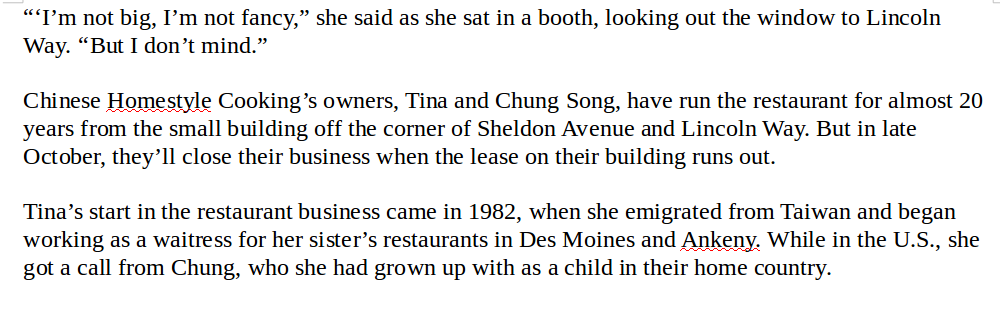
\includegraphics[width=0.9\textwidth]{Example.png}
\\ \footnotesize{Source: Ames Tribune \url{http://goo.gl/zvx9Uw}}
\begin{enumerate}
\item What is the main event of this text? \pause
\item What is "Chinese Homestyle Cooking" referring to? \pause
\item What is the relationship between "Chinese Homestyle cooking" and Tina? \pause
\item Is Lincoln Way something related to President Lincoln?
\end{enumerate}
\end{frame}

\begin{frame}
\frametitle{NLP tasks: Word Collocations and Concordances}
\begin{itemize}
\item Task: compiling lists of words, or word sequences occuring in documents.
\item Simplest and least ambiguous form of language processing. 
\item Can get to more advanced collocations beyond surface forms.
\item Established methods already exist for collecting different kinds of collocations
\end{itemize}
\end{frame}

\begin{frame}
\frametitle{NLP tasks: Pattern Extraction}
\begin{itemize}
\item Task: Extract the language patterns that exist in textual data. 
\item Regular expressions are very useful for this
\item More advanced methods (which rely on machine learning) exist to extract unknown patterns from unstructured text documents.
\end{itemize}
\end{frame}

\begin{frame}
\frametitle{NLP tasks: POS Tagging}
\framesubtitle{What is the big deal about automatic tagging?}
\begin{itemize}
\item Task: Given a sequence of words, return the POS tags for each word.
\item An example problem: What is the best tag for a word in a context?
\begin{itemize}
\item I wish to cite this work. 
\\ PRP/I  VBP/wish  TO/to  VB/cite  DT/this  NN/work ./.
\item He has a wish.
\\ PRP/He  VBZ/has  DT/a  NN/wish ./. 
\end{itemize}
\item Largely considered solved for English, but there are still issues if we go beyond typical newspaper language (e.g., tagging speech or tweets). Still an unsolved problem for several languages.
\end{itemize}
\end{frame}

\begin{frame}
\frametitle{NLP tasks: Parsing}
\begin{itemize}
\item Task: Construct the syntactic structure of a given sentence.
\item Two kinds of trees can be generated in NLP: Phrase structure tree (Constituency tree), Dependency tree
\item PST: shows parse structure in terms of Noun Phrases, Verb Phrases, Prep. Phrases etc.
\item Dependency Tree: shows relations between words in a sentence in terms of a pre-defined set of relations
\item Very active area of current research, for multiple languages.
\item Important note: POS tagging errors can carry over and affect parser efficiency. 
\end{itemize}
\end{frame}

\begin{frame}
\frametitle{NLP tasks: Parsing}
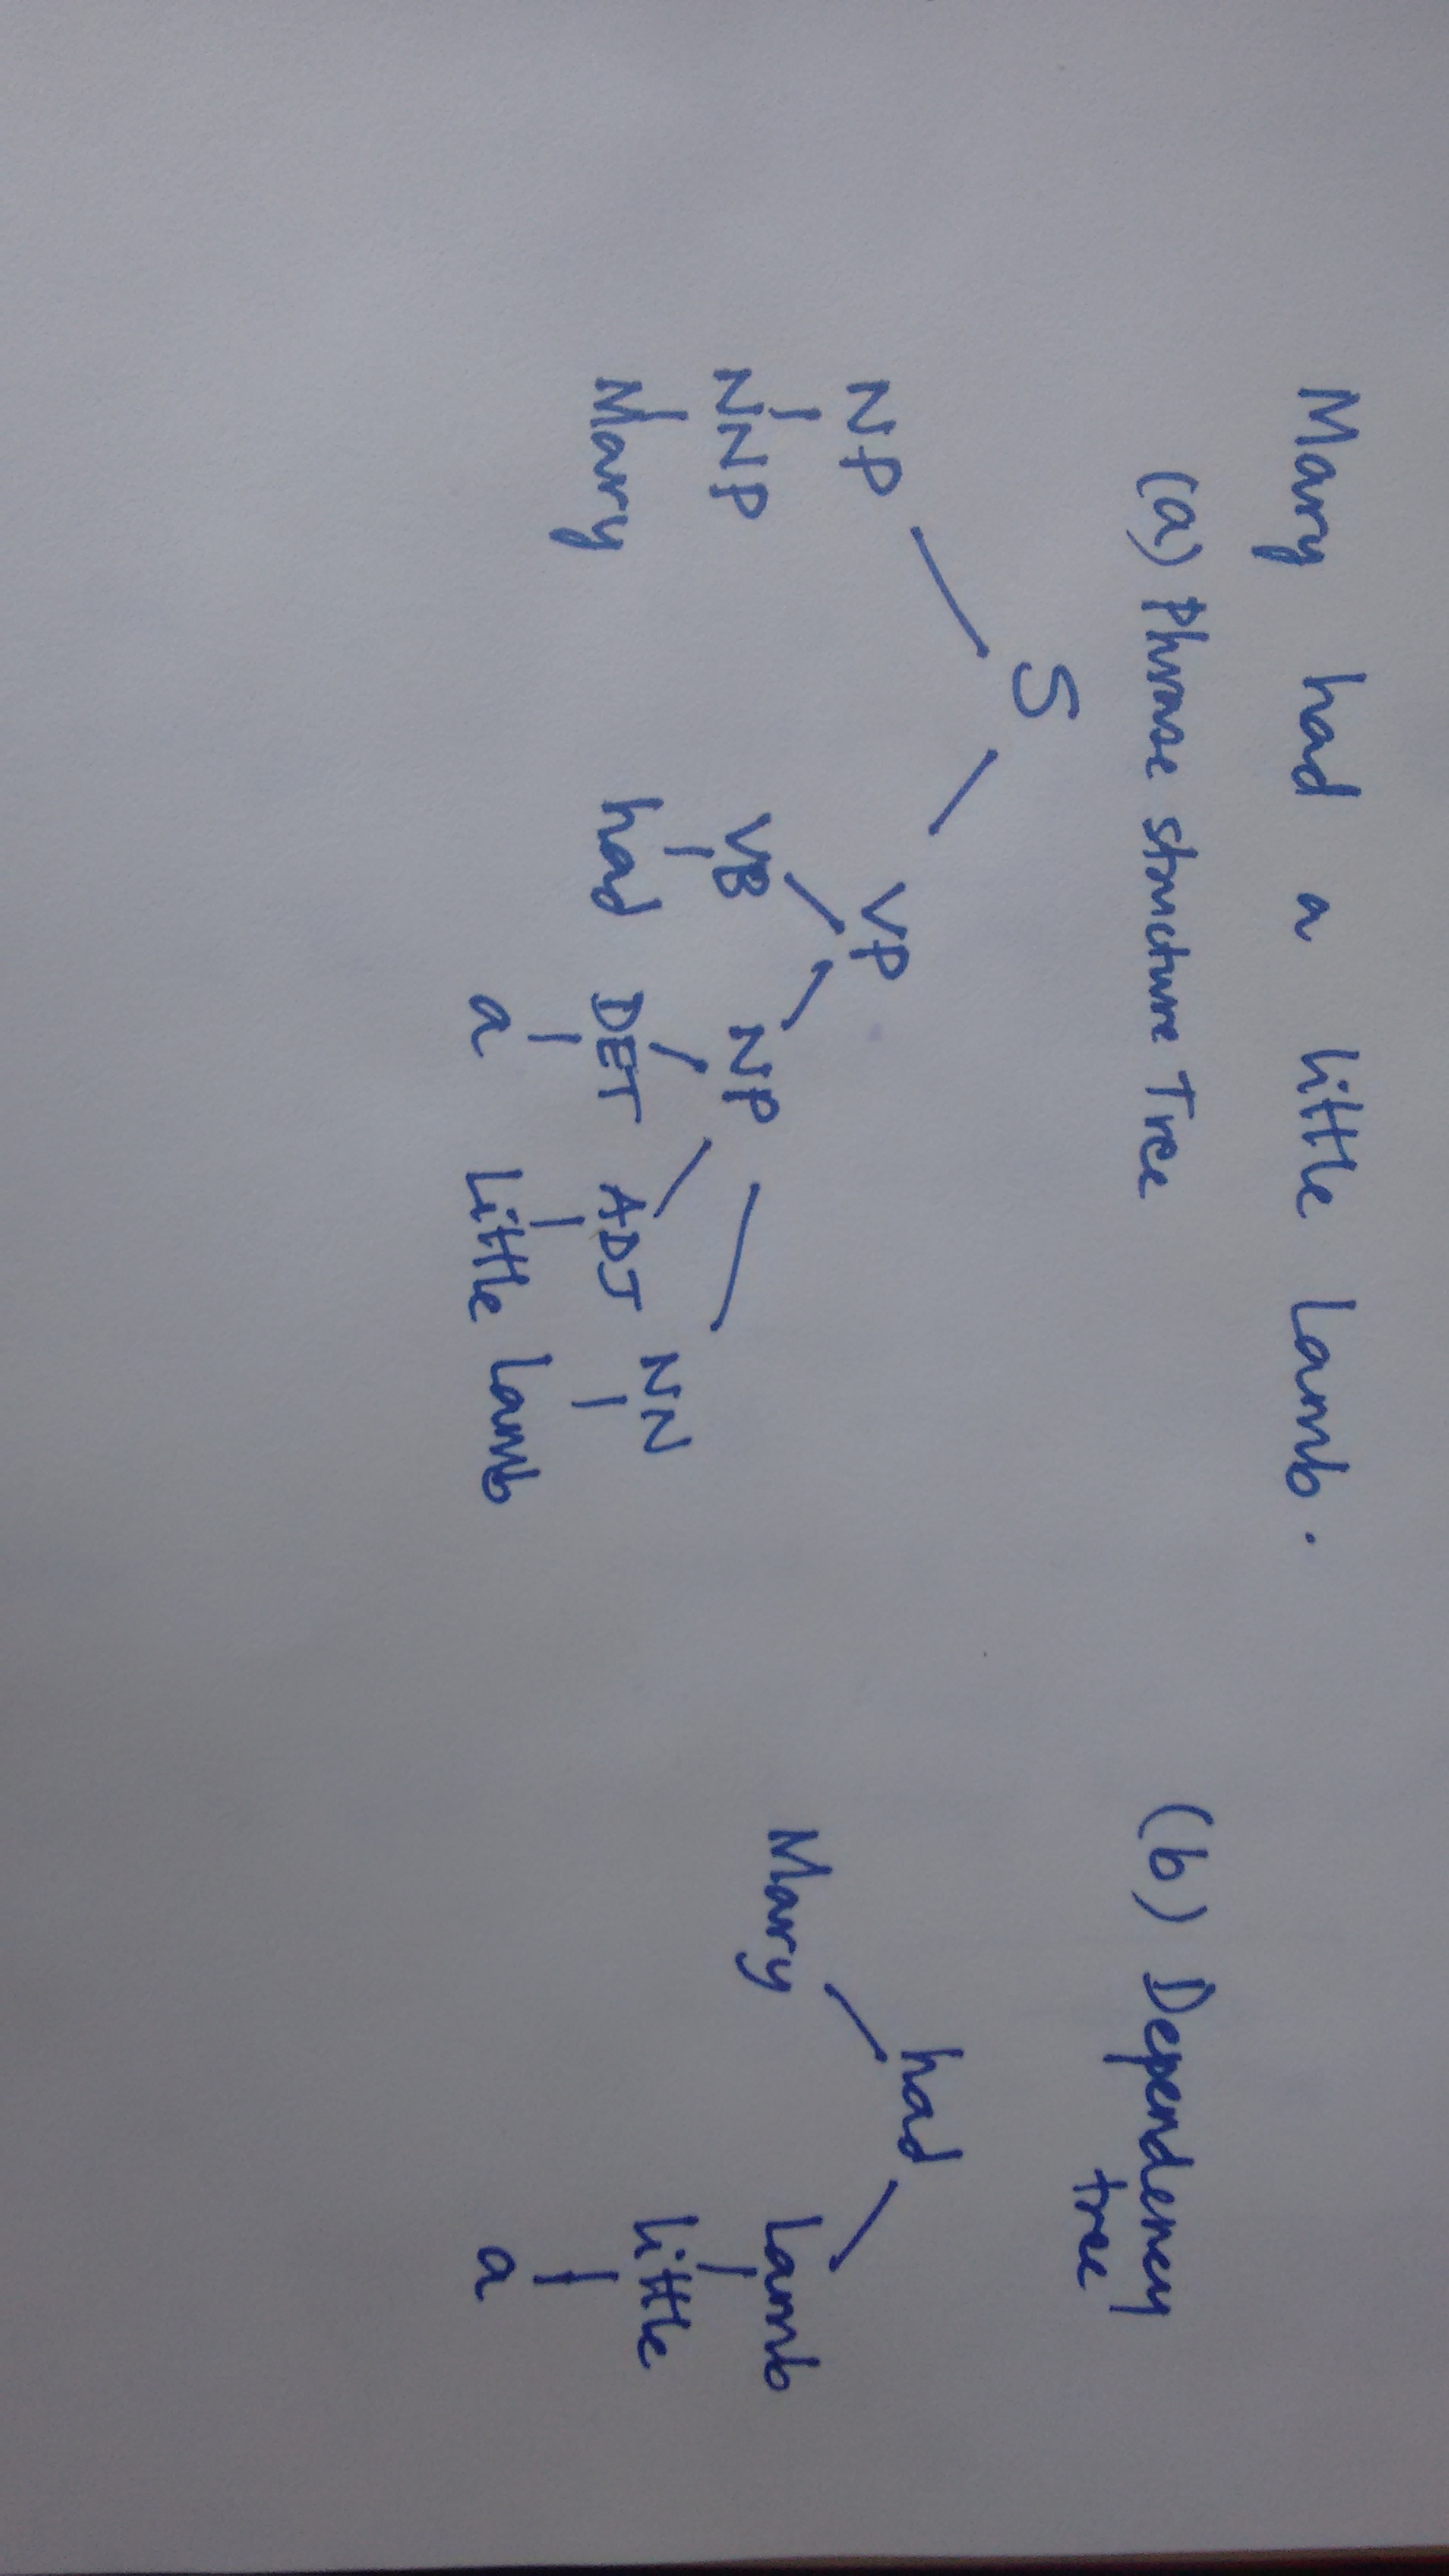
\includegraphics[width=0.6\textwidth,angle=90]{parses.jpg}
\end{frame}

\begin{frame}
\frametitle{NLP tasks: Word Sense Disambiguation}
\begin{itemize}
\item Task: For words that can have multiple meanings, what is the right sense of the word in a given sentence? 
\item Example: "Let us go inside, it is cold" vs "I have cold and cough"
\item Very important for applications such as machine translation, information retrieval
\item Good progress for English WSD. One of the active areas of research in the field.
\end{itemize}
\end{frame}

\begin{frame}
\frametitle{NLP tasks: Named Entity Recognition}
\begin{itemize}
\item Task: Identify and classify named entities (e.g., person names, organization names, locations etc.,) 
\item Application: Information extraction from text 
\item Some NER is domain specific (biomedical NER, financial NER etc)
\item Current methods of NER: hand-crafted or automatically compiled lists + statistical machine learning models
\item Active area of research for English and other languages. 
\end{itemize}
\end{frame}

\begin{frame}
\frametitle{NLP tasks: Semantic Role Labeling}
\begin{itemize}
\item SRL is all about doing a "semantic parse" of a sentence. The task here is to identify argument structure of a sentence and thematic roles of different entities.
\item Example: (source: \url{http://www.cs.upc.edu/~srlconll/})
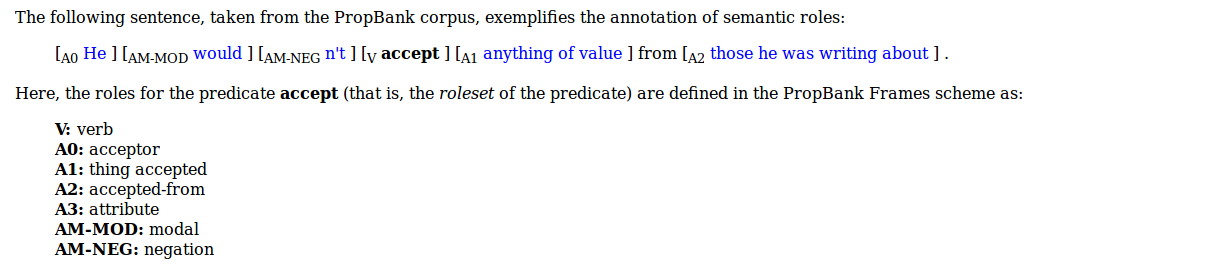
\includegraphics[width=\textwidth]{SRL.png}
\item Active area of research. Still hard, but making progress.
\end{itemize}
\end{frame}

\begin{frame}
\frametitle{NLP tasks: Discourse Analysis}
\begin{itemize}
\item Task: Given a text (more than one sentence), analyze the relationships between sentences, identify what pronouns refer to what nouns, how is the same entity referred in different ways (Barack Obama, Obama, The President and so on).
\item Application: Text summarization, Question-Answering, Essay scoring etc.
\item Hard problem, but active research topic and hence, making good progress
\end{itemize}
\end{frame}

\begin{frame}
\frametitle{NLP tasks: Text - Speech interface}
\begin{itemize}
\item Text to speech conversion, Speech to text conversion
\item Traditionally studied separately under Speech processing. Not a part of NLP courses generally.
\item Difficult task, but lot of improvement in speech recognition happened in the recent past, partly due to "deep learning" methods
\item You can easily incorporate speech recognition into your Python code now, without writing any speech related code yourself! 
\end{itemize}
\end{frame}

\begin{frame}
\frametitle{NLP tasks: Entailment and Paraphrasing}
\begin{itemize}
\item Tasks: Analyzing if the meaning of a sentence is entailed in another sentence, if both sentences are paraphrases of each other etc.,
\item Uses: question answering, information extraction, summarization etc.
\item Still very hard. Most of the research is with English.. so we don't know if that is even harder for several other languages.
\end{itemize}

\end{frame}

\begin{frame}
\frametitle{NLP tasks: Language Generation}
\begin{itemize}
\item Task: Generate text automatically.
\item Texts should be grammatically and semantically correct. Should be human like.
\item One of the toughest problems in NLP. 
\item Example 1: Create weather reports, match summaries, reports etc. automatically (without human intervention!)
\item arria.com is a NLG company that does this successfully for English.
\item There are some software libraries that support the development of NLG systems for some languages currently.
\end{itemize}
\end{frame}

%questions?
\begin{frame}
\frametitle{Question Time}
Where in CALL applications are the following tasks relevant:
\begin{itemize}
\item Paraphrase identification %short answer scoring?
\item Natural Language Generation %giving feedback dynamically?
\item Text to Speech conversion
\item Speech to Text conversion
\item Named Entity Recognition %short answer scoring
\end{itemize}
\end{frame}

\begin{frame}
\frametitle{NLP: References, Resources etc}
\begin{itemize}
\item Access to various publications: \url{http://aclweb.org/anthology/} \\ (Almost all major publication venues in the field are open-access!)\item Information about resources for different languages: ACL Wiki \url{http://www.aclweb.org/aclwiki}
\item Know about other NLP courses around the world etc: ACLWeb again
\end{itemize}
\end{frame}

\begin{frame}
\begin{center}
Assignment 1 description
\\ (Deadline: 10 September)
\\ On Blackboard as PDF
\end{center}
\end{frame}

\begin{frame}
\frametitle{Next Week}
\begin{itemize}
\item To Do: 
\begin{enumerate}
\item Start revising your programming concepts. Look at the notes you made in the previous course.
\item Go through Radev's course lectures: Week1 and last three lectures from Week 3.
\item Read Chapter 1 in Jurafsky and Martin book
\item Python users: You can start with Chapter 1 in the book if you want to do some stuff on your own.
\end{enumerate}
\item Next week: 
\begin{enumerate}
\item Programming review and practice. Come prepared to work either on your laptops or lab machines.
\item Setting up Perl and Python programming environments on lab machines or personal laptops
\end{enumerate}
\end{itemize}
\end{frame}

\begin{frame}
\frametitle{}
\begin{center}
Programming Project - Demos
\end{center}
\end{frame}
\end{document}

\begin{frame}
\frametitle{Problem solving time!}
Read this problem, and try to find an answer: \url{http://goo.gl/kplOJ3}
\pause
\\ Solution: \url{http://goo.gl/Iy8xVK}
\end{frame}

\end{document}
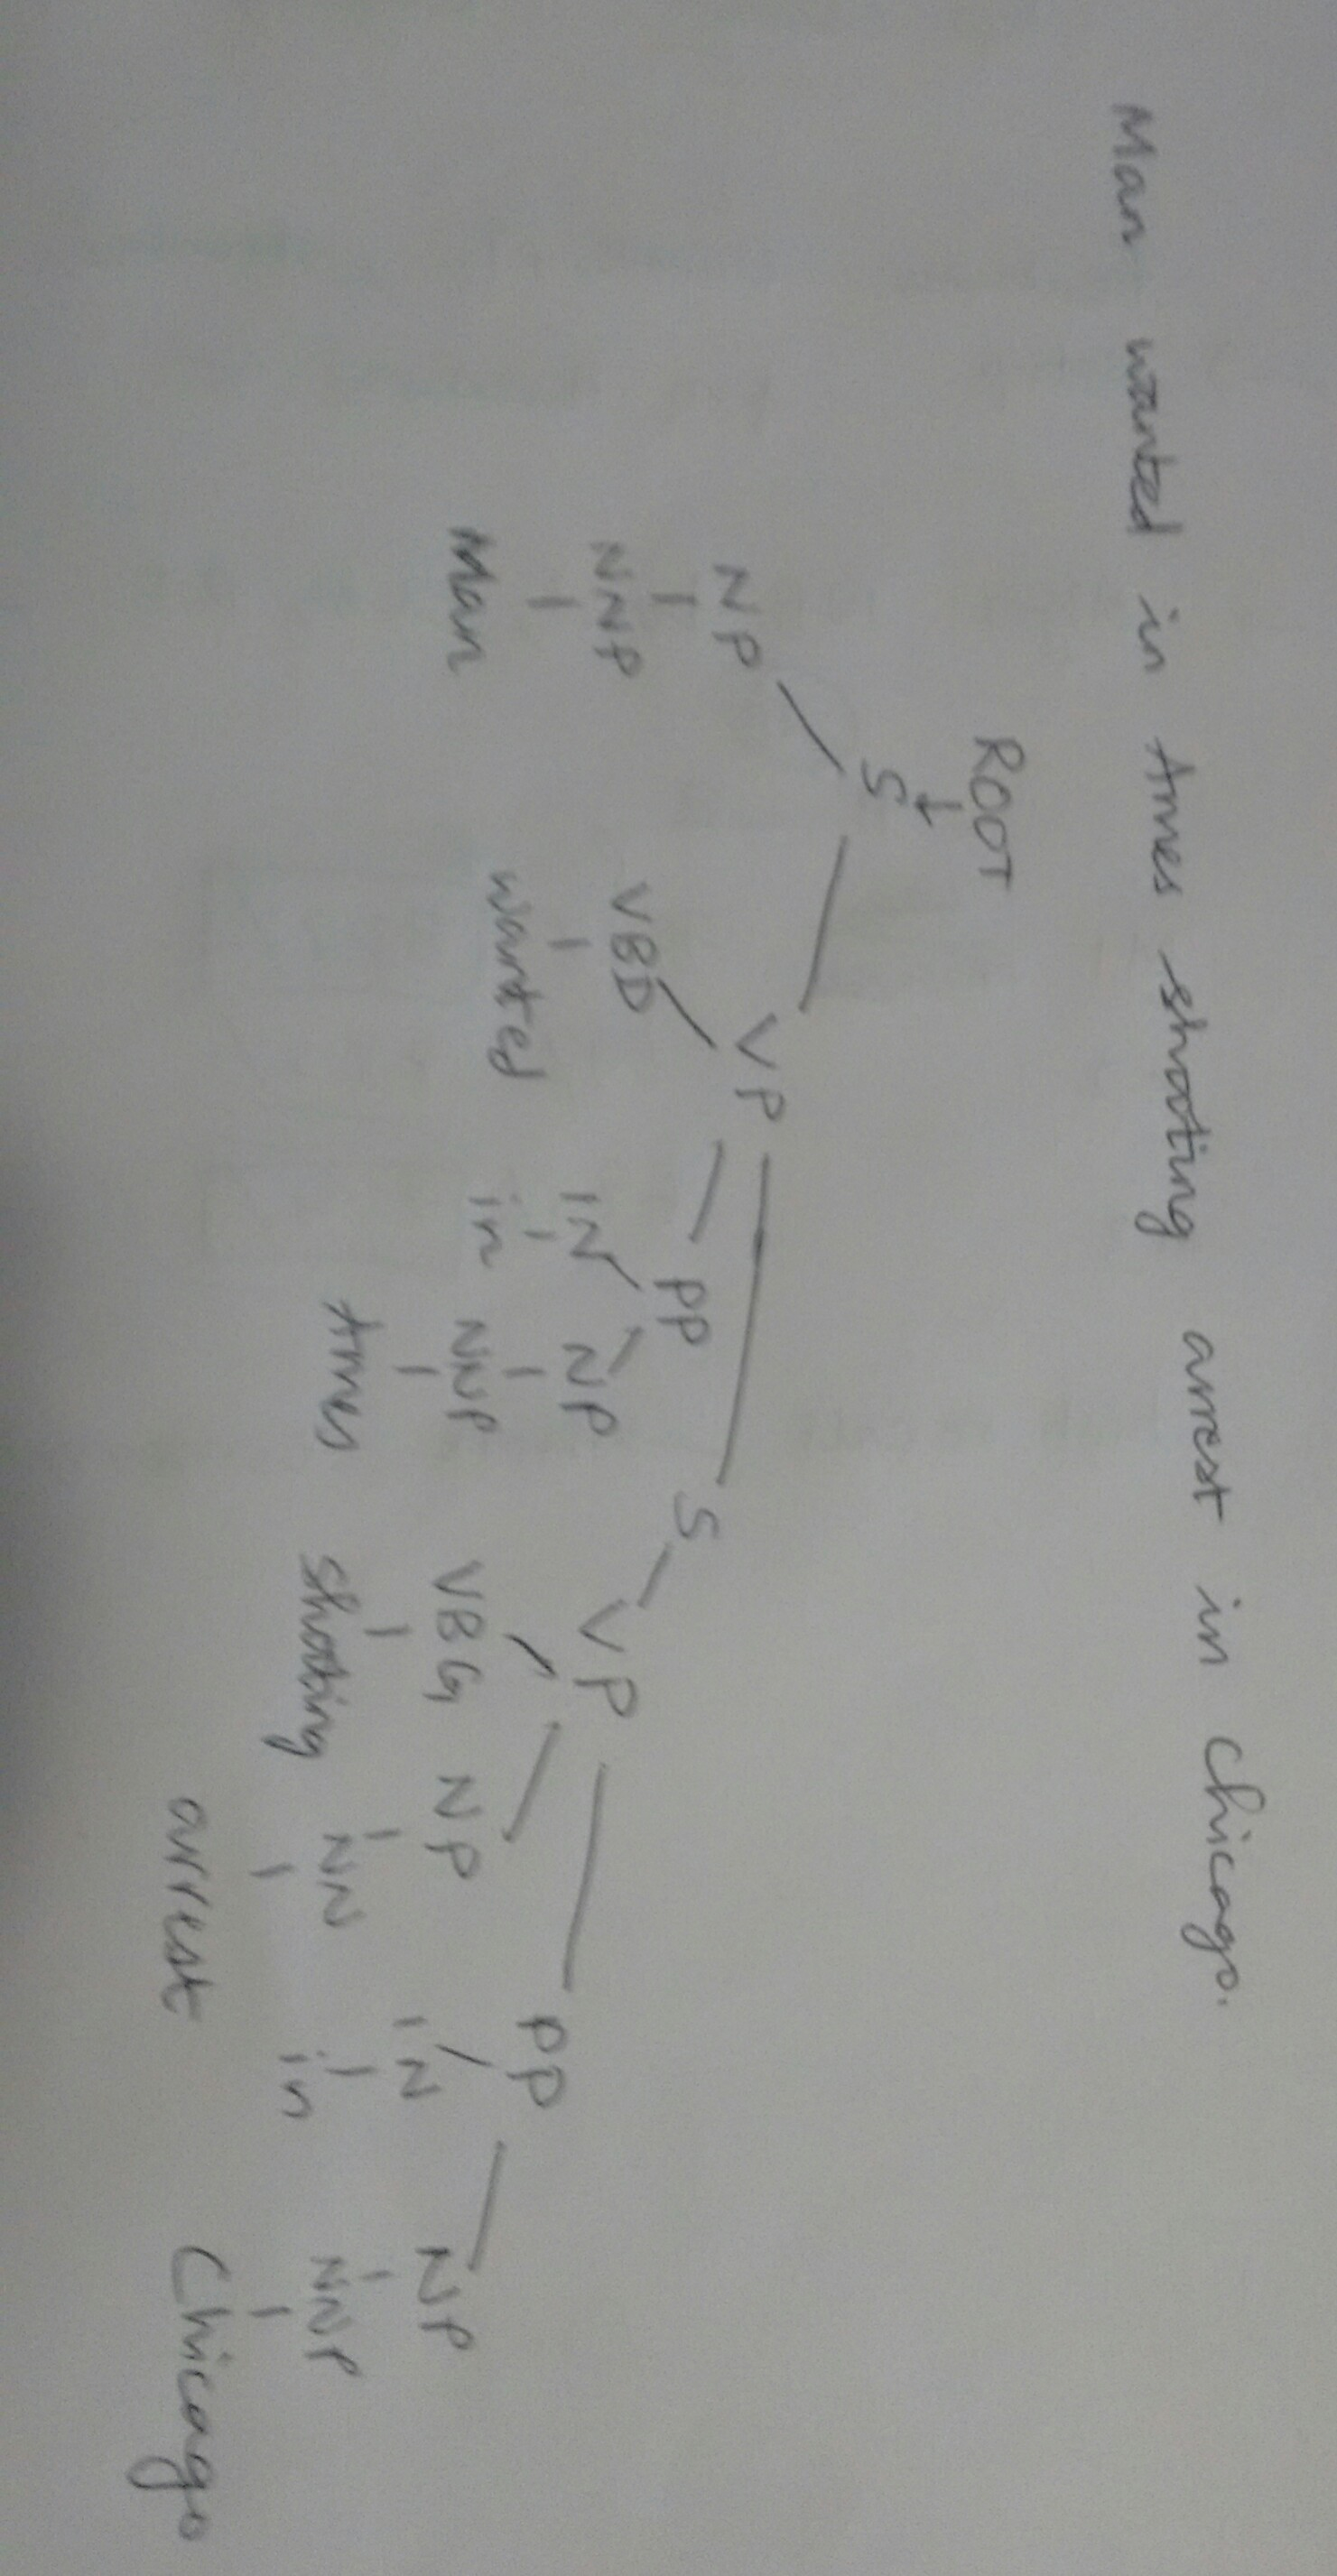
\includegraphics[width=0.5\textwidth,angle =90]{headline-parse.jpg}
%Man wanted in Ames shooting arrest in Chicago. - recent headline
%actual sentence: A Fort Dodge man wanted in a shooting in Ames was arrested in Chicago.
%Water main break floods Campustown
%Water main break flooded Campustown
